\chapter{شبیه‌سازی}
\noindent
\textbf{
\textit{
توصیف روند شبیه‌سازی سخت‌افزار و گام‌های اجرایی، مشاهدهٔ ورودی‌ها و خروجی‌های اصلی و میانی، مقایسه با مقادیر حاصل از اجرای کد نرم‌افزاری (مدل طلایی)، توصیف مراحل اجزای الگوریتم به همراه شکل موج‌ها، نحوهٔ عملکرد 
\lr{Testbench}
}
}
\pagebreak

\section{توضیح روند شبیه‌سازی سخت‌افزار و گام‌های اجرایی}
برای شبیه‌سازی سخت‌افزاری کد 
\lr{verilog}
الگوریتم 
\lr{Skein}
را در محیط شبیه‌سازی 
\lr{Modelsim}
اجرا کردیم. گام‌های اجرایی به صورت کلی برای شبیه‌سازی کد سخت‌افزاری موارد زیر بود. 
\begin{itemize}
\item
مطالعه کد الگوریتم و تعیین ورودی‌ها
\item
نوشتن Testbench
\item
اجرای کد در محیط Modelsim با Testbench های مختلف
\item
گرفتن Waveform و مقادیر خروجی (اصلی و میانی)
\end{itemize}
\section{مشاهدهٔ ورودی‌ها و خروجی‌های اصلی و میانی}
در ادامه ابتدا کد های Testbench اجرا شده بر الگوریتم و سپس Waveform
های حاصله و در انتها خروجی‌ها به صورت متنی آورده می‌شود.

\subsection{توضیح نحوهٔ عملکرد Testbench}
در ادامه ابتدا کد verilog نوشته‌شده برای هر Testbench آورده  و سپس توضیحاتی دربارهٔ آن ایراد شده است. 

 \subsubsection{\lr{Testbench 1}}
\begin{code}
//First Testbench
module top;
    reg clk = 1'b0;
    reg [511:0] midstate = 72;
    reg [95:0] data = "hello" ;
    reg [31:0] nonce = 13;
    wire [511:0] hash;
    always #1 clk = !clk;

    skein512 skein(clk, midstate , data ,nonce , hash);
    
    initial
  begin
        #300 data = "how are you?";
 		#300 data = "bye";
        #5000 $stop;
  end
endmodule
\end{code}

در این testbench ابتدا مقادیر ورودی‌ها تنظیم می‌شوند
به ترتیب به ازای clock  و midstate و data و nonce مقادیر 0 و 72 و 
"hello"
 و 13 تنظیم می‌شوند

پس از 300 واحد زمانی مقدار data تغییر می‌کند و به
"how are you?"
 تبدیل می‌شود و پس از 300 واحد زمانی دیگر به 
 "bye"
 تغییر می‌کند.
ترتیب و مقدار hash در بخش مربوط به آن آمده است.

\subsubsection{\lr{Testbench 2}}
\begin{code}
//Second Testbench
module top;
    reg clk = 1'b0;
    reg [511:0] midstate = 72;
    reg [95:0] data = "hello" ;
    reg [31:0] nonce = 23;
    wire [511:0] hash;
    always #1 clk = !clk;

    skein512 skein(clk, midstate , data ,nonce , hash);
    
    initial
  begin
        #300 data = "how are you?";
  		#300 data = "bye";
        #5000 $stop;
  end
endmodule
\end{code}

در این testbench نیز ابتدا مقادیر ورودی‌ها تنظیم می‌شوند،
به ترتیب به ازای clock  و midstate و data و nonce مقادیر 0 و 72 و 
"hello"
و 23 تنظیم می‌شوند
پس از 300 واحد زمانی مقدار data تغییر می‌کند و به 
"how are you?"
تبدیل می‌شود و پس از 300 واحد زمانی دیگر به 
"bye"
 تغییر می‌کند.
ترتیب و مقدار hash در بخش مربوط به آن آمده است
تنها تفاوت این بخش و بخش قبلی در مقادیر ورودی nonce است که از 13 به 23 تغییر داده شده است.


\subsubsection{\lr{Testbench 3}}
\begin{code}
//Third Testbench
module top;
    reg clk = 1'b0;
    reg [511:0] midstate = 72;
    reg [95:0] data = "still awake" ;
    reg [31:0] nonce = 23;
    wire [511:0] hash;
    always #1 clk = !clk;

    skein512 skein(clk, midstate , data ,nonce , hash);
    
    initial
  begin
        #300 data = "working";
        #6000 $stop;
  end
endmodule
\end{code}
در این testbench ابتدا مقادیر ورودی ها تنظیم می‌شوند،
به ترتیب به ازای clock  و midstate و data و nonce مقادیر 0 و 72 و 
"still awake"
 و 23 تنظیم می‌شوند
پس از 300 واحد زمانی مقدار data تغییر می‌کند وبه 
"working"
 تبدیل می‌شود.
ترتیب و مقدار hash در بخش مربوط به آن آمده است.
در این بخش با تغییر مقادیر اولیه و ثانویه data خروجی ها را با قسمت قبل مقایسه کردیم.

\subsection{مقادیر خروجی‌های حاصل از Testbench ها}

\subsubsection{\lr{Waveform 1}}
\begin{figure}[H]
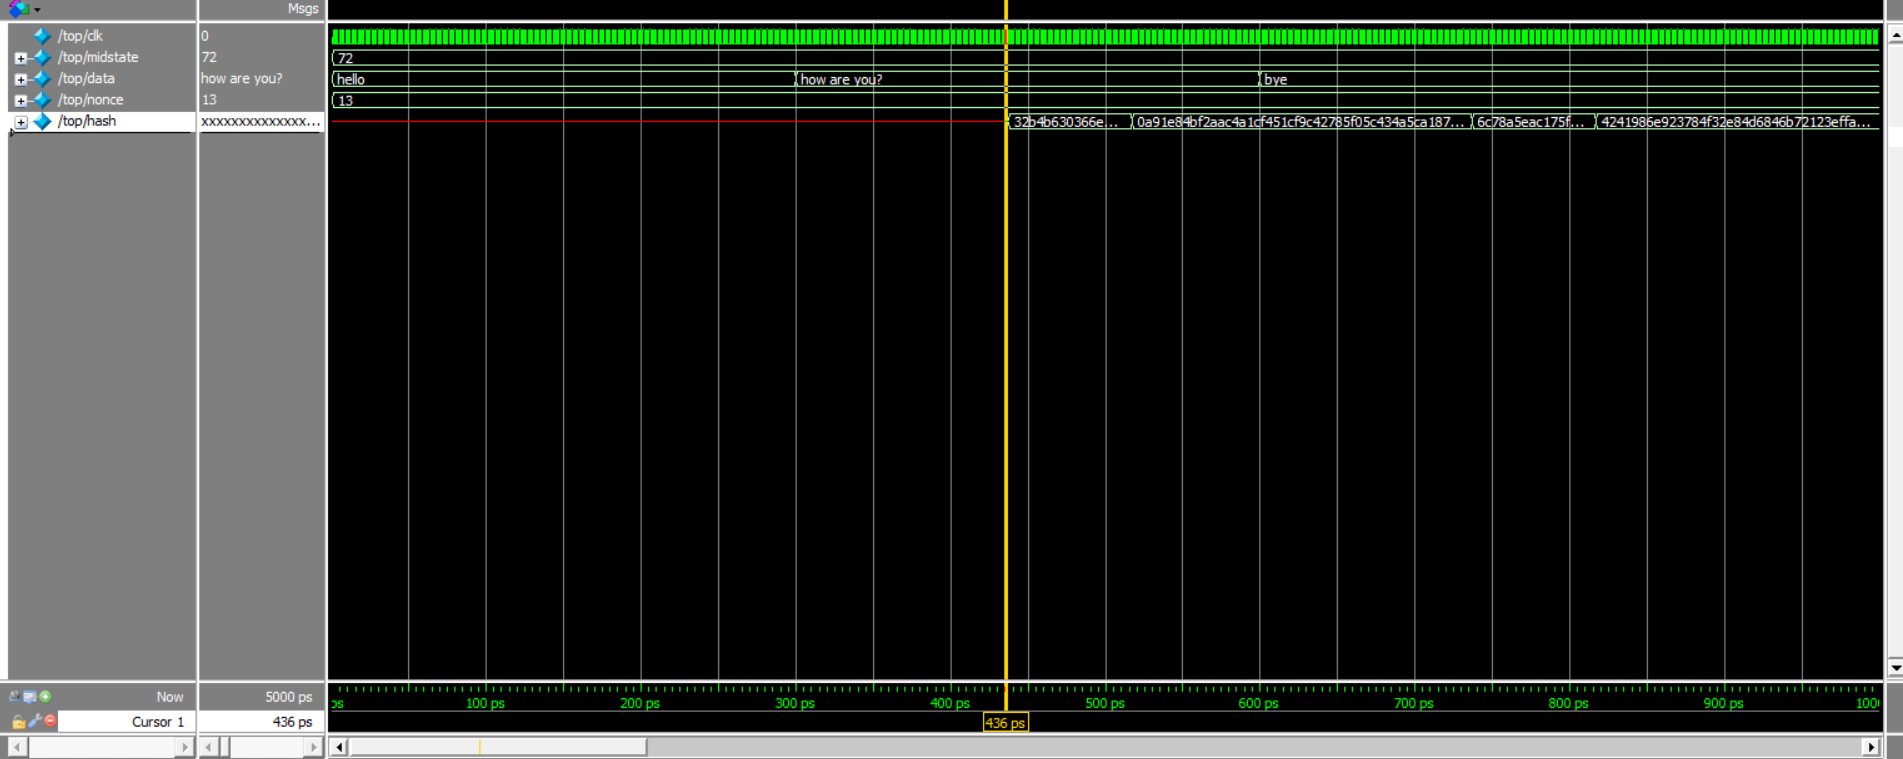
\includegraphics[width = \textwidth]{figs/simulation/1.png}
\caption{شبیه‌سازی با \lr{Testbench 1}}
\label{simulation_1}
\end{figure}

\subsubsection{\lr{Waveform 2}}
\begin{figure}[H]
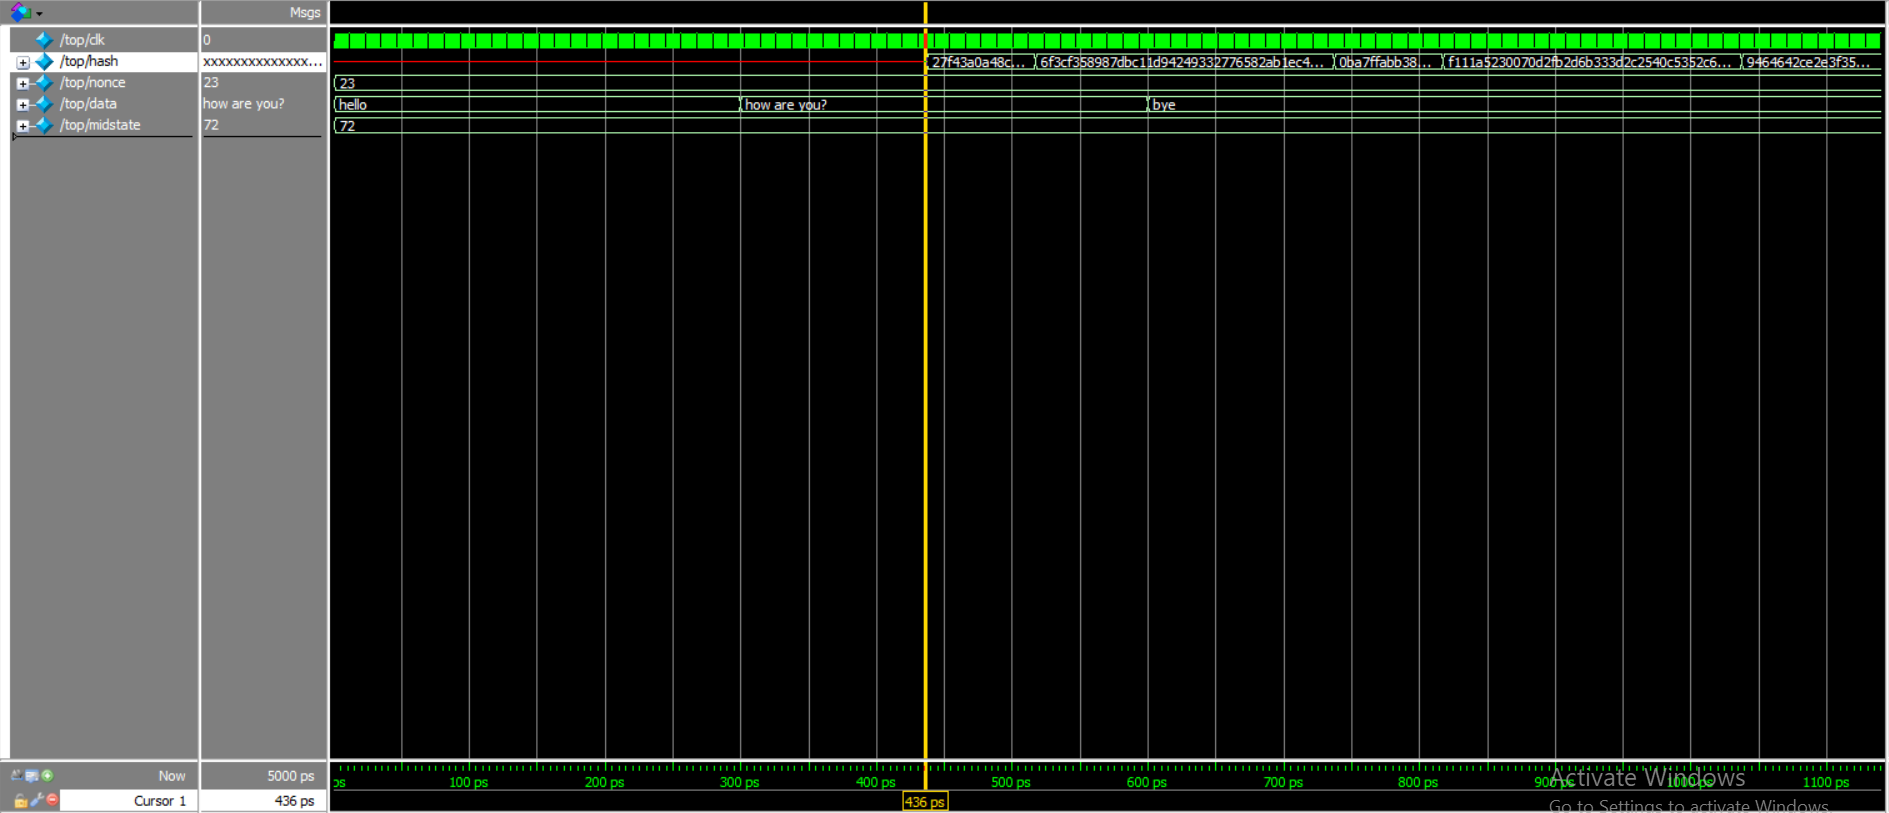
\includegraphics[width = \textwidth]{figs/simulation/2.png}
\caption{شبیه‌سازی با \lr{Testbench 2}}
\label{simulation_2}
\end{figure}

\subsubsection{\lr{Waveform 3}}
\begin{figure}[H]
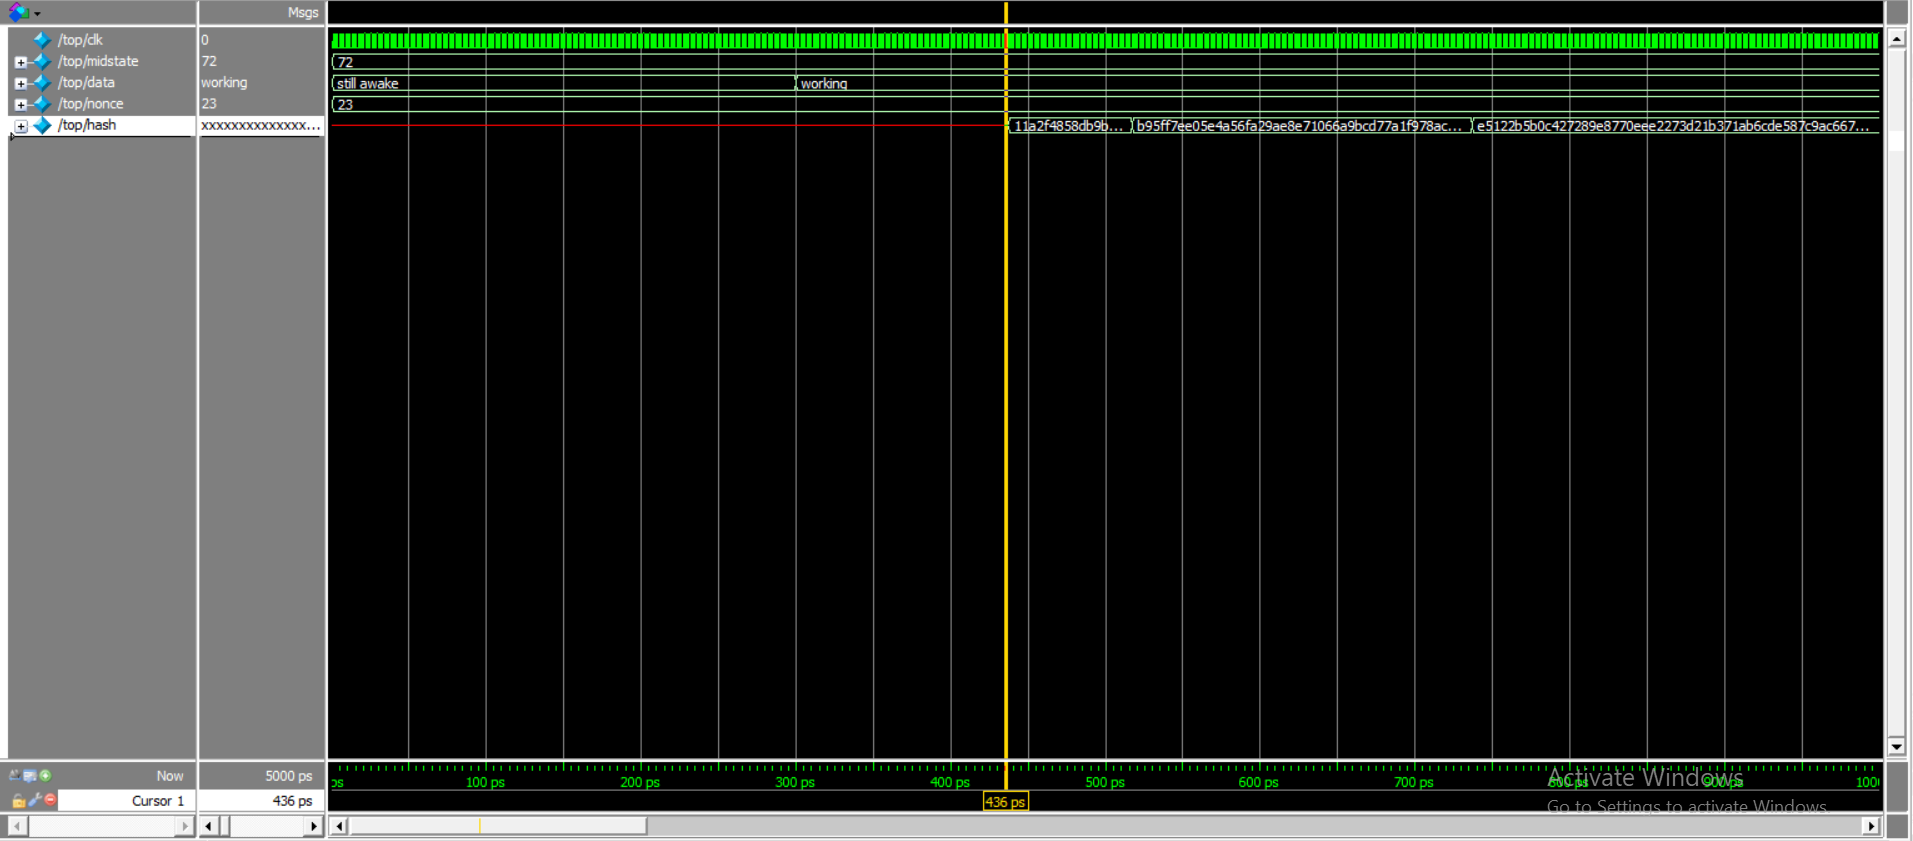
\includegraphics[width = \textwidth]{figs/simulation/3.png}
\caption{شبیه‌سازی با \lr{Testbench 3}}
\label{simulation_3}
\end{figure}

\subsection{جدول خروجی‌های هش برای Testbench ها}

\subsubsection{\lr{Output 1}}

\lr{
\begin{table}[H]
\resizebox{\textwidth}{!}{%
\begin{tabular}{@{}llll@{}}
\toprule
Final & Hash                                                                                                                                                                        & Time(clk) & Data \\ \midrule
False & \begin{tabular}[c]{@{}l@{}}32b4b630366ea0d126796328ad99cf0dbb95b4b3b08bdac2c9965ab01993886\\ 499e4a150a5b7f93ac75eaad9c70cc3b2e7147887c5953849c9ddc96b2cbfa417\end{tabular} & 436       & hello         \\
True  & \begin{tabular}[c]{@{}l@{}}0a91e84bf2aac4a1cf451cf9c42785f05c434a5ca1876c64382210c0c2102aa5\\ 2fa8064a67e7510a670d0558a54efbc789d6c9b0198258d85e797e82bfc0f26e\end{tabular} &           & hello         \\
False & \begin{tabular}[c]{@{}l@{}}6c78a5eac175f4456c22f40253f9c2b877a1f8dc177ba179f9778f468c7ce8b3\\ 79a8d2f259227c9e2320eff4040ff3d81461a0ae93cb5d6fd4fa0b6c37334df9\end{tabular} &           & how are you?  \\
True  & \begin{tabular}[c]{@{}l@{}}4241986e923784f32e84d6846b72123effa16f143d874cbeefc815dd972e15d9b\\ 3591d2d409de47c364dd6d7676ce4050220b28a762fa1dc39099280459c8e74\end{tabular} &           & how are you?  \\
True  & \begin{tabular}[c]{@{}l@{}}aed5a975b556508072d512af282bbe56877874bd463a786544e3406875931cf\\ 8e5f8a7e823193eeed2904bc00ac5d3e7f81d8162667b7ac171f1fbd92dcda7e5\end{tabular} &           & bye           \\ \bottomrule
\end{tabular}%
}
\rl{
\caption{مقادیر درهم‌سازی و زمان با توجه به \lr{Testbench 1}}}
\label{table_1}
\end{table}
}


\subsubsection{\lr{Output 2}}

\lr{
% Please add the following required packages to your document preamble:
% \usepackage{booktabs}
% \usepackage{graphicx}
\begin{table}[H]
\resizebox{\textwidth}{!}{%
\begin{tabular}{@{}llll@{}}
\toprule
Final & Hash                                                                                                                                                                        & Time(clk) & \textbf{Data} \\ \midrule
False & \begin{tabular}[c]{@{}l@{}}27f43a0a48c65a7b90d2915a252b4ad97063a43818089082a95c2dbe5148ed7\\ 0c07604d0cdf5310df8b18c3f368b83516f7f4195b435d53900d5fe31c8f6ee20\end{tabular} & 436       & hello         \\
True  & \begin{tabular}[c]{@{}l@{}}6f3cf358987dbc11d94249332776582ab1ec4e81ce512fa28e5f8d77dd9c6e04\\ 224c88f2b28bda6c0becf728f5e45c60bf20f22ca4f08a030f38db131694ce30\end{tabular} &           & hello         \\
False & \begin{tabular}[c]{@{}l@{}}0ba7ffabb38454cdf8f29d2b33ef4a9a3ab103e20d9eeb8b55ef36707ced67952\\ 80c9695df1d5d1072939177e48994faaf226161fb3998b90254f5bc0e51ba2b\end{tabular} &           & how are you?  \\
True  & \begin{tabular}[c]{@{}l@{}}f111a5230070d2fb2d6b333d2c2540c5352c61585f4e5ba3b485c7a33400a04\\ 17ff4898cba78441791013f571a1aafdf287d597b5162937d194ff67f6620f270\end{tabular} &           & how are you?  \\
True  & \begin{tabular}[c]{@{}l@{}}9464642ce2e3f35da6af64bb4b5ffda92151870f81c98934946ff4921364cf80c\\ d134e927accac3ebe7d35d0e1ac9bf4933063a0a182a53d84f0c65e588e1b24\end{tabular} &           & bye           \\ \bottomrule
\end{tabular}%
}
\rl{
\caption{مقادیر درهم‌سازی و زمان با توجه به \lr{Testbench 2}}}
\label{table_2}
\end{table}
}


